\section{总结}

图数据库的关键特性在于, 将用户提交的增删查改需求转化为图论问题, 进一步使用(可利用向量处理器并行加速的)图论算法进行求解, 及时地将结果反馈给用户(和其它存储节点)。

在分布式应用场景中, 图数据库的架构和传统关系型数据库, 如\cref{fig:graphDB-DistArchtec}所示, 并没有十分明显的差异。这意味着适用于关系型数据库的策略, 如读写分离、负载均衡, 也同样地适用于图数据库的具体部署。因此可以说,图数据库在产业界的实际应用从一开始就有了好的基础。

\begin{figure}[H]
	\centering
	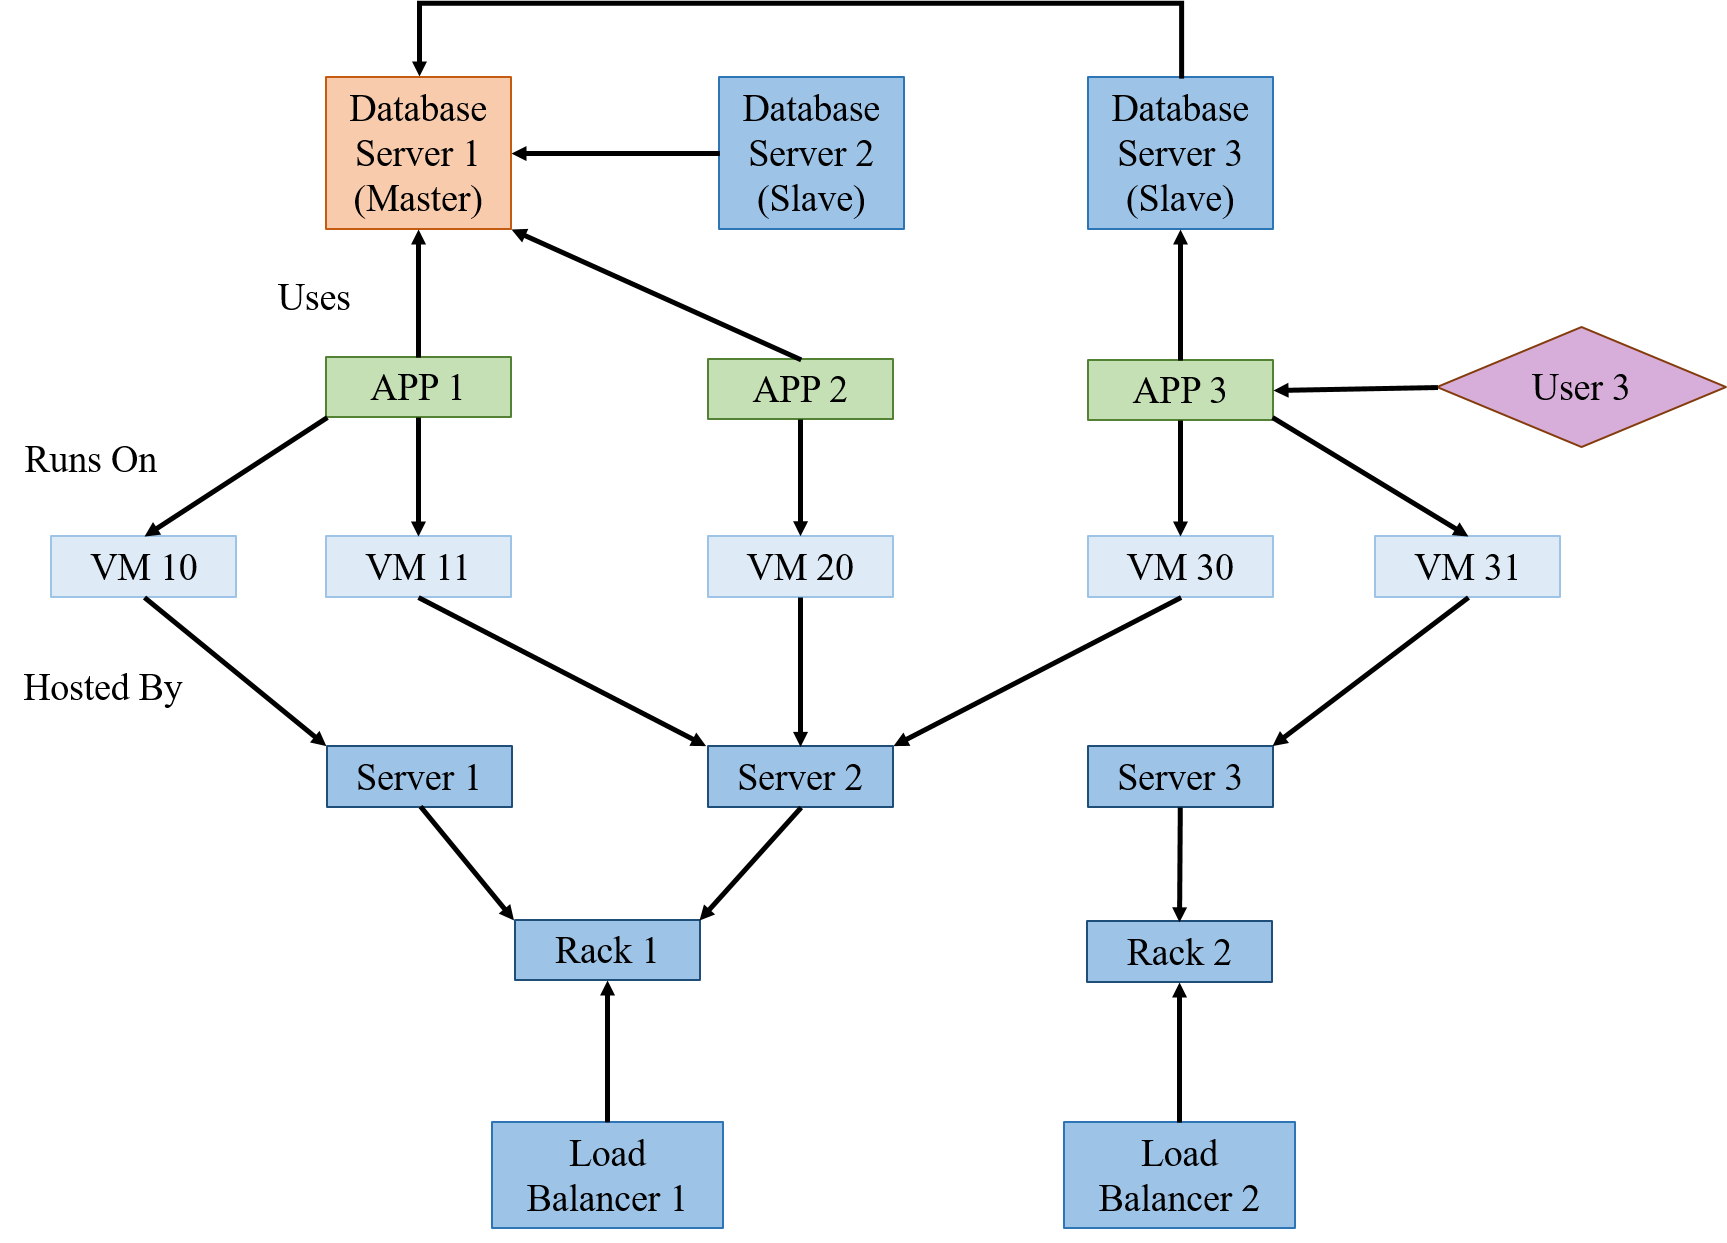
\includegraphics[width=\textwidth]{images/27.png}
	\caption{分布式图数据库的架构}
	\label{fig:graphDB-DistArchtec}
\end{figure}

可以预见的是, 随着查询语言标准化的深入推进, 图数据库也会像关系型数据库那样, 发展出对用户和应用开发者都十分友好的一系列产品——遵循一定标准而又提供个性化的支持, 甚至和其它类型的数据库构成多模型数据库。毋庸置疑,图数据库的未来是可期的。 
